\section{Reduced image complexity (v3)}\label{sec:osm_v3}
The implication of utilizing both satellite images and expert knowledge (in terms of a path loss model) requires further investigation and explorations. In particular, it is of interest to effectively reduce the model complexity to enable a more transparent inference of the prediction capability. Additionally, and possibly, more importantly, it is of great interest to validate the approach by using inherently different data sources. 

In the work \cite{Thrane2020DeepKnowledge}, the proposed approach is validated using simplified geographical images and additional drive test data. More specifically, this includes the use of so-called \emph{OpenStreetMap} data to supply the needed information for the used images. Furthermore, to enable generalization and interpolation between inherently different data sources, some changes were conducted to the features. The approach of this is visualized in Fig. \ref{fig:version3_architecture_figure}.

\begin{figure*}
    \centering
    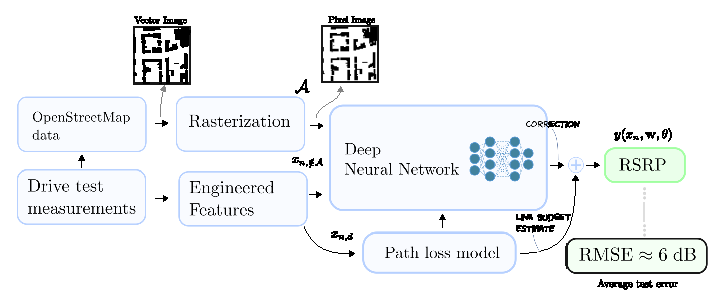
\includegraphics{chapters/part_pathloss/osm_images_paper/figures/version3_architecture_figure.eps}
    \caption{Architecture is set to utilize images provided by \gls{osm} instead of satellite images}
    \label{fig:version3_architecture_figure}
\end{figure*}




\subsection{German measurements}

The experimental measurements of the previously used drive test data (See appendix \ref{app:drive_test_study_2017}, \cite{1xf4-eg98-19}) is appended with data from Dortmund, Germany \cite{SliwaEmpiricalNetworks}. The dataset contains measurements from multiple \glspl{mno} in different propagation scenarios at different operating frequencies. The essential characteristics can be seen in Table \ref{tab:drive_test_data_total}. The fundamental characteristics of the data allow for engineering the relevant features required for applying the proposed \gls{dl} model.

\begin{table*}[h]
\footnotesize
\begin{tabular}{@{}llll@{}}
\toprule
Dataset      & Samples & MNOs & Frequencies  [MHz]       \\ \midrule
DK Campus    & $57586$   & $1$    & $[811, 2630]$ \\
GER Campus   & $8579$    & $3$    & $[850, 860, 1815, 1845, 1865, 2630]$                   \\
GER Urban    & $11921$   & $3$    &  $[850, 860, 1845, 1865, 2630, 2650, 2680]$ \\
GER Suburban & $27152$   & $3$    &  $[850, 860, 1815, 1845, 1865,2630]$                   \\
GER Highway  & $20662$   & $3$    & $[850, 860, 870, 950, 1815, 1845, 1865,2630]$                    \\ \midrule
Total        & $125900$  &      &                     \\ \bottomrule
\end{tabular}
\vspace{1em}
\caption{Additional drive test data is available for training and testing consisting of various transmission frequencies.}\label{tab:drive_test_data_total}
\end{table*}

\subsection{Methodology}

Upon initial prototyping of the proposed method, it was found that the general features of \gls{gnss} positions, e.g. latitude and longitude coordinates caused severe extrapolation issues. More specifically, the model attempted to interpolate between the coordinates. The importance of the coordinates to the prediction of \gls{rsrp} caused the model to learn latent features of spatial importance. When evaluating the methodology in a different region (significant difference in latitude and longitude coordinates), the trained model would then provide a wrong interpretation of the spatial features by interpolating between coordinates. For this reason, a few changes to the formalized of the required engineered features were made. More specifically this resulted in

\begin{equation}
    x_n = [v, d, \Delta_\text{lat}, \Delta_\text{lon},  f_c, \mathcal{A}]
\end{equation}

Where $v$ is the velocity of the vehicle, $d$ is the distance in $3$D, $\Delta_\text{lat}$, $\Delta_\text{lon}$ are the difference in latitude and longitude between the receiver and the \gls{enb} respectively. $f_c$ is the carrier frequency in MHz, and $\mathcal{A}$ is the new simplified image.

The image was constructed similarly as \emph{v1} and \emph{v2}, using a \gls{roi} and a rotation towards the transmitter. Instead of the rotation causing the transmitter to be direction south (down) in the image, the image was rotated such that a direct path is to the east (right) in the image. Any performance gains did not cause this change, but rather ease of implementation. An example of such an image can be seen in Fig. \ref{fig:roi_image_preperation}. The area spanned by the image was adjusted to find the optimum use of the images. The rasterized image was kept constant at a size of $64 \times 64$ pixels. The images were extracted with the tool as documented in \cite{SliwaLightweightNetworks}. Data augmentation, as discussed in Section \ref{sec:training_v2}, was applied similarly.


\begin{figure}
    \centering
    
\includegraphics{chapters/part_pathloss/osm_images_paper/figures/map_to_image.eps}
    \caption{The \gls{roi} was determined around the measurement position spanning a variable size of area covered.}
    \label{fig:roi_image_preperation}
\end{figure}

\subsection{Model Architecture}

The model architecture was kept similar to the one used in \emph{v2} embedding expert knowledge of path loss. A change to model complexity was necessary due to the simplification of 1) the engineered features and 2) the geographical images. The general idea of the model architecture is identical to that of Fig. \ref{fig:combined_model_approach} and Fig. \ref{fig:satellite_model_setup_v2}. The reduction in model complexity resulted in a significant increase of the hyper-parameters scanned and the automatization hereof. A Bayesian optimization scheme was applied to find the most probable hyper-parameters given the weight space provided by the final test error \cite{YuHyper-ParameterApplications, wandb}. Over $500$ experiments of different hyper-parameters and combinations hereof was conducted, resulting in a large model complexity reduction. An example of the hyper-parameter experiments can be found in Fig. \ref{fig:hyper-paramters_scan}. The final achieved hyper-parameters can be found in Table \ref{tab:hyper-parameters}.

Specifically, a reduction of convolutional filters can be observed. For instance, the first layer of the \gls{cnn} is reduced with $\approx 170$ filters compared to \emph{v2}. Furthermore, the size of the fully-connected layers processing the engineered features has also seen a reduction from $200$ to $32$. Additionally, the last \gls{nn} sub-module has been reduced from $200$ to $16$. This reduction has reduced not only the memory footprint of the proposed model but also the training performance and thus the resulting inference performance. Specifically, the model complexity reduction has resulted in sub-millisecond prediction times (accelerated with a GPU). 

\begin{figure*}
    \centering
    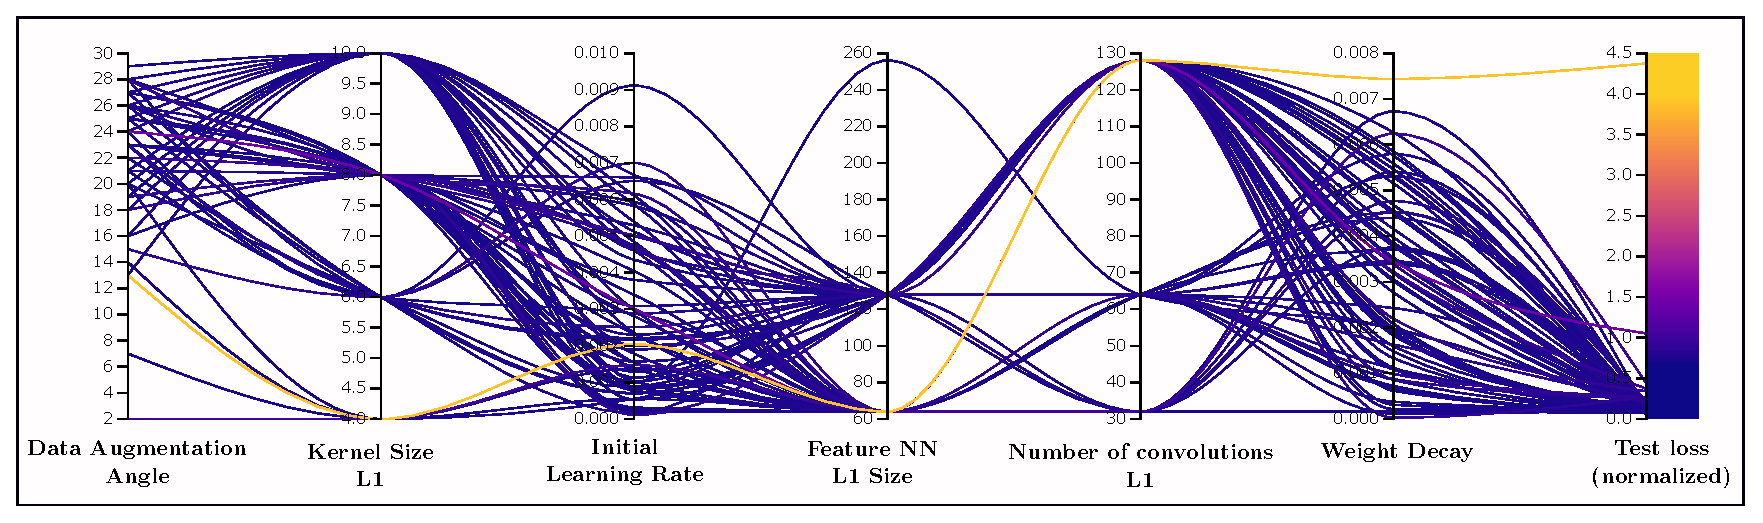
\includegraphics{chapters/part_pathloss/osm_images_paper/figures/hyperparameter_scan.eps}
    \caption{Bayesian optimization applied during hyper-parameter scan \cite{wandb}.}
    \label{fig:hyper-paramters_scan}
\end{figure*}


\begin{table}[]
    \centering
    \footnotesize
    \caption{Hyper-parameters for the deep neural network model.}\label{tab:hyper-parameters}
    \begin{tabular}{@{}lll@{}}
    \toprule
    \textbf{Parameter}          & \textbf{Value}                &  \\ \midrule
    Weight decay                & 8e-4                          &  \\
    Learning rate               & 1e-3                          &  \\
    Filters                     & [32, 32, 10, 1]               &  \\
    Kernel size                 & [(5,5), (3,3), (3,3), (2,2)]  &  \\
    Max pooling                 & [2, 2, 2, 2]                  &  \\
    Feature NN layer size       & [32, 32]                      &  \\
    Output NN layer size        & [16, 16]                      & \\
    Image augmentation angle    & 20                            & \\
    Image size                  & $64~\text{px} \times 64~\text{px}$                & \\
    Batch size                  & 12                            &  \\ \bottomrule
\end{tabular}
\end{table}

\newpage
\newpage


\subsection{Comparative results}
The results of utilizing simple geographical images instead of the satellite images can be seen in Fig. \ref{fig:model_comparison_access}. The overall performance can be seen to be identical to that of \emph{v2} on the same test set. A slight decrease at 811 MHz in performance is observed, however with a slight difference in the standard deviation across several version of the final trained models. Similar performance at $2630$ MHz was achieved.

\begin{figure}[h]
    \centering
    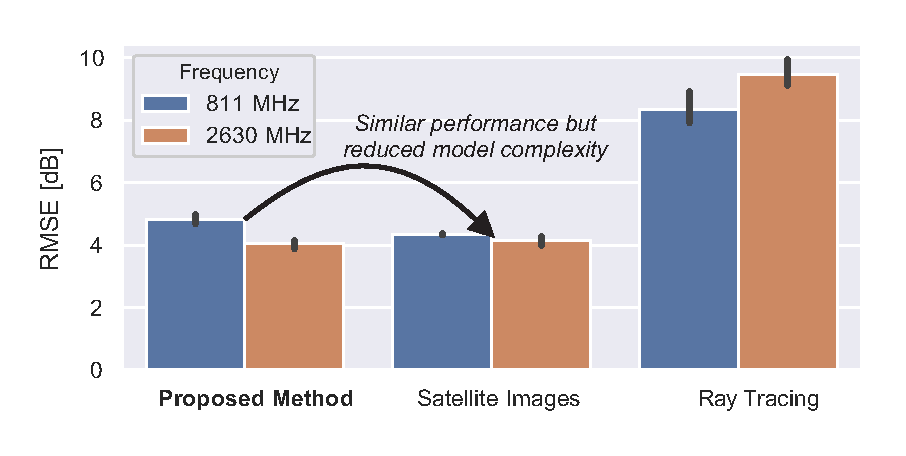
\includegraphics{chapters/part_pathloss/osm_images_paper/figures/model_comparison_access.eps}
    \caption{Comparison of simple \gls{osm} images with satellite images and ray-tracing.}
    \label{fig:model_comparison_access}
\end{figure}


To further explore the performance across all of the data subsets, a cross-validation approach was employed. Specifically, this entailed training on the majority of subsets while keeping one scenario for testing, repeated for all subsets. For instance, when refereed to the performance of \texttt{GER Campus} - it is trained on all other subsets of data excluding the \texttt{GER Campus} subset. The generalization gap for all subsets can be seen in Fig. \ref{fig:generalization_gap}. The figure shows the difference between the test and training error for each training epoch; in other words, how well the trained model performs on the remaining subset. If close to zero a generalization across the data subset is achieved. It can be seen that the \texttt{GER Campus} subset achieves by far the best generalization performance. The worst generalization is achieved for the \texttt{DK campus} subset. Both the \texttt{GER suburban} and \texttt{GER urban} subset achieved similar performance.

\begin{figure}[h]
    \centering
    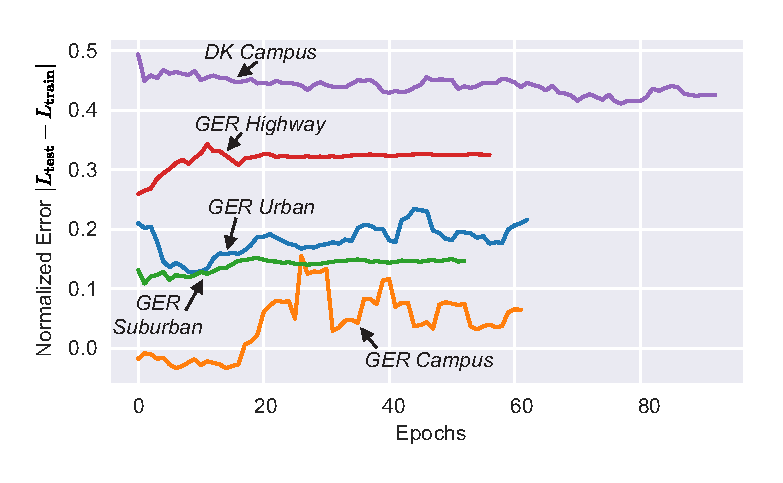
\includegraphics{chapters/part_pathloss/osm_images_paper/figures/training_test_error_crossvalidation_diff.eps}
    \caption{Generalization gap for all subsets.}
    \label{fig:generalization_gap}
\end{figure}

The performance is also evaluated in terms of \gls{rmse} (see \ref{eq:rmse}). This can be observed in Fig. \ref{fig:rmse_boxplot_osm} (lower is better). The cross-validated performance is shown for all subsets. The \gls{rmse} is computed for all mini-batches of samples, thus the figure shows the average \gls{rmse} across all mini-batches and the resulting standard deviation. Furthermore, outliers are also displayed. The best performance is achieved on the \texttt{GER campus} subset with a \gls{rmse} of $6.3$ dB and $\sigma = 3.6$ dB. The worst performance is seen on the \texttt{GER Highway} subset, with an \gls{rmse} of $9.7$ dB and $\sigma = 1.2$ dB.


\begin{figure}[h]
    \centering
    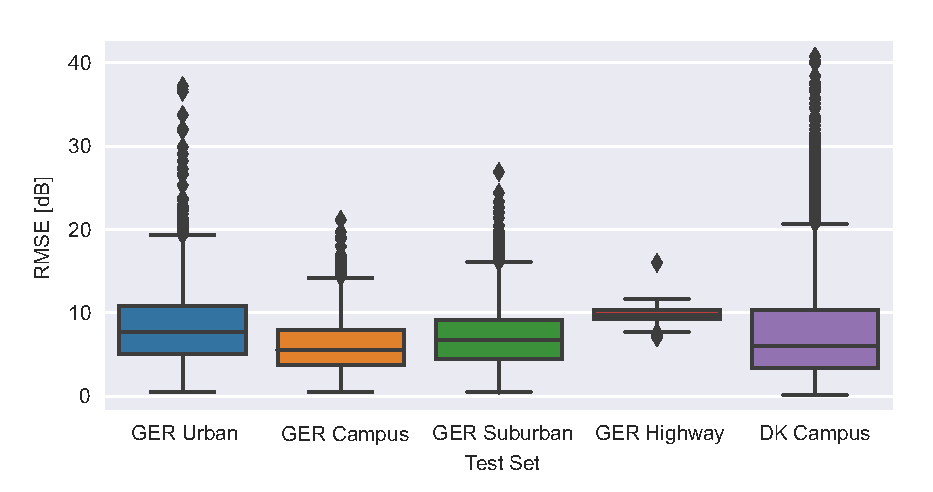
\includegraphics{chapters/part_pathloss/osm_images_paper/figures/RMSE_boxplot.eps}
    \caption{Cross-validation results of all data subsets. Each subset is evaluated using a model trained on the remainder of the subsets.}
    \label{fig:rmse_boxplot_osm}
\end{figure}

\subsection{Image distance results}
As a result of the reduced model complexity, additional exploration of the importance of spatial dependency has been completed. This has resulted in the comparison of so-called \emph{full-size} images instead of the \emph{regular} \gls{roi} images (centered around the measurement coordinate). The \emph{full-size} images consider not only the receiver location but also the transmitter location. In other words, both positions are within the spanned \emph{full-size} image. Thus, if the antenna separation distance increase, the area spanned by the image increase.  \emph{Regular} images have a constant area covered by the image regardless of antenna separation distance. A so-called \emph{violin} plot is found in Fig. \ref{fig:rmse_violin_image_comparison}. The figure shows the estimation of the kernel density provided by batch-wise \gls{rmse} computation. The distribution and range of using \emph{full-size} images are noticeably different than using the \emph{regular} images spanning 250 meters. More so, the number of outliers (and the range) increased. Using \emph{regular} images resulted in an \gls{rmse} of $6.3$ dB while an \gls{rmse} of $7.3$ dB was achieved using the \emph{full-size} images



\begin{figure}[h]
    \centering
    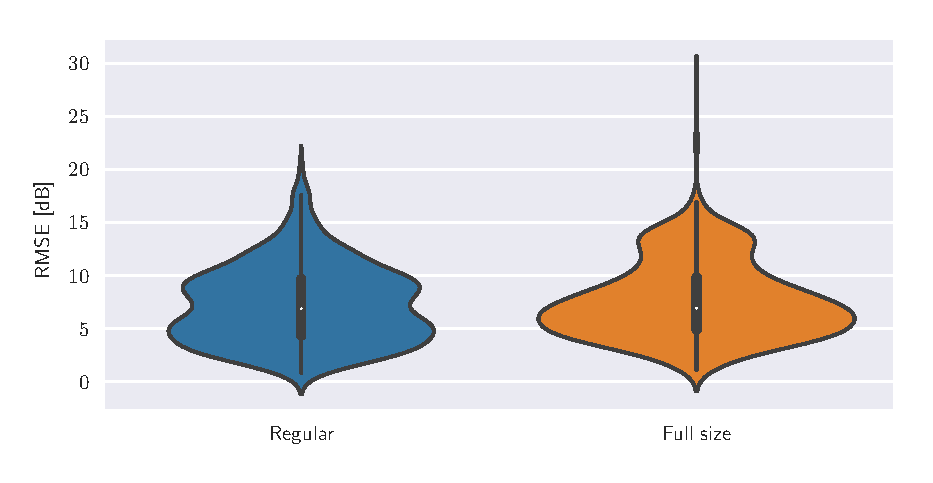
\includegraphics{chapters/part_pathloss/osm_images_paper/figures/RMSE_violin.eps}
    \caption{Performance comparison of varying the area spanned by the images. Evaluated on \texttt{GER Campus}, trained on the remainder.}
    \label{fig:rmse_violin_image_comparison}
\end{figure}


The impact of the area spanned by the \gls{roi} is evaluated in Fig. \ref{fig:boxplot_ci_image_distance}. The area spanned by the images are varied, while the pixel size of the image is kept constant. The performance is evaluated concerning the \texttt{GER Campus} subset, with a model trained on the remainder of the subsets. The best performing images were found spanning a distance of $250-300$ meters with similar predictive performance. Decreasing the distance spanned by the images offers a slight increase in \gls{rmse}. The same is observed for increasing the distance spanned by the images.

\begin{figure}
    \centering
    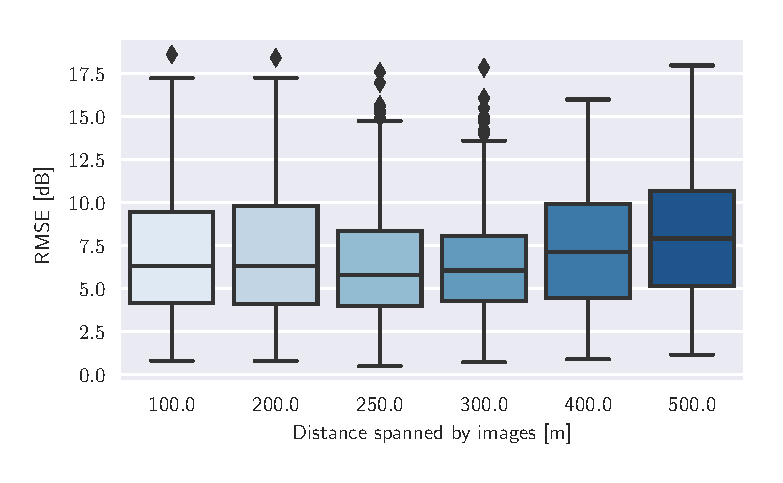
\includegraphics{chapters/part_pathloss/osm_images_paper/figures/boxplot_ci_image_distance.eps}
    \caption{Performance comparison of utilizing different distances for the images. The performance is with respect to the \texttt{GER Campus} subset, trained on the remainder.}
    \label{fig:boxplot_ci_image_distance}
\end{figure}

\subsection{Heatmap generation}

The trained models can effectively extrapolate and interpolate measurements in the area of the originated drive tests. An example of this for 2630 MHz can be seen in Fig. \ref{fig:osm_heatmap}. The model is trained on the entirety of the data points in the \texttt{DK Campus} subset. A grid of features is generated for all latitude and longitude coordinates in the area of interest. The model is then evaluated for the generated features. The results show a feasible range of predicted \gls{rsrp} values, in the range of $-80$ to $-140$ dBm. Furthermore, an increase in \gls{rsrp} is seen near the \gls{enb} location. 

\begin{figure}[!h]
    \centering
    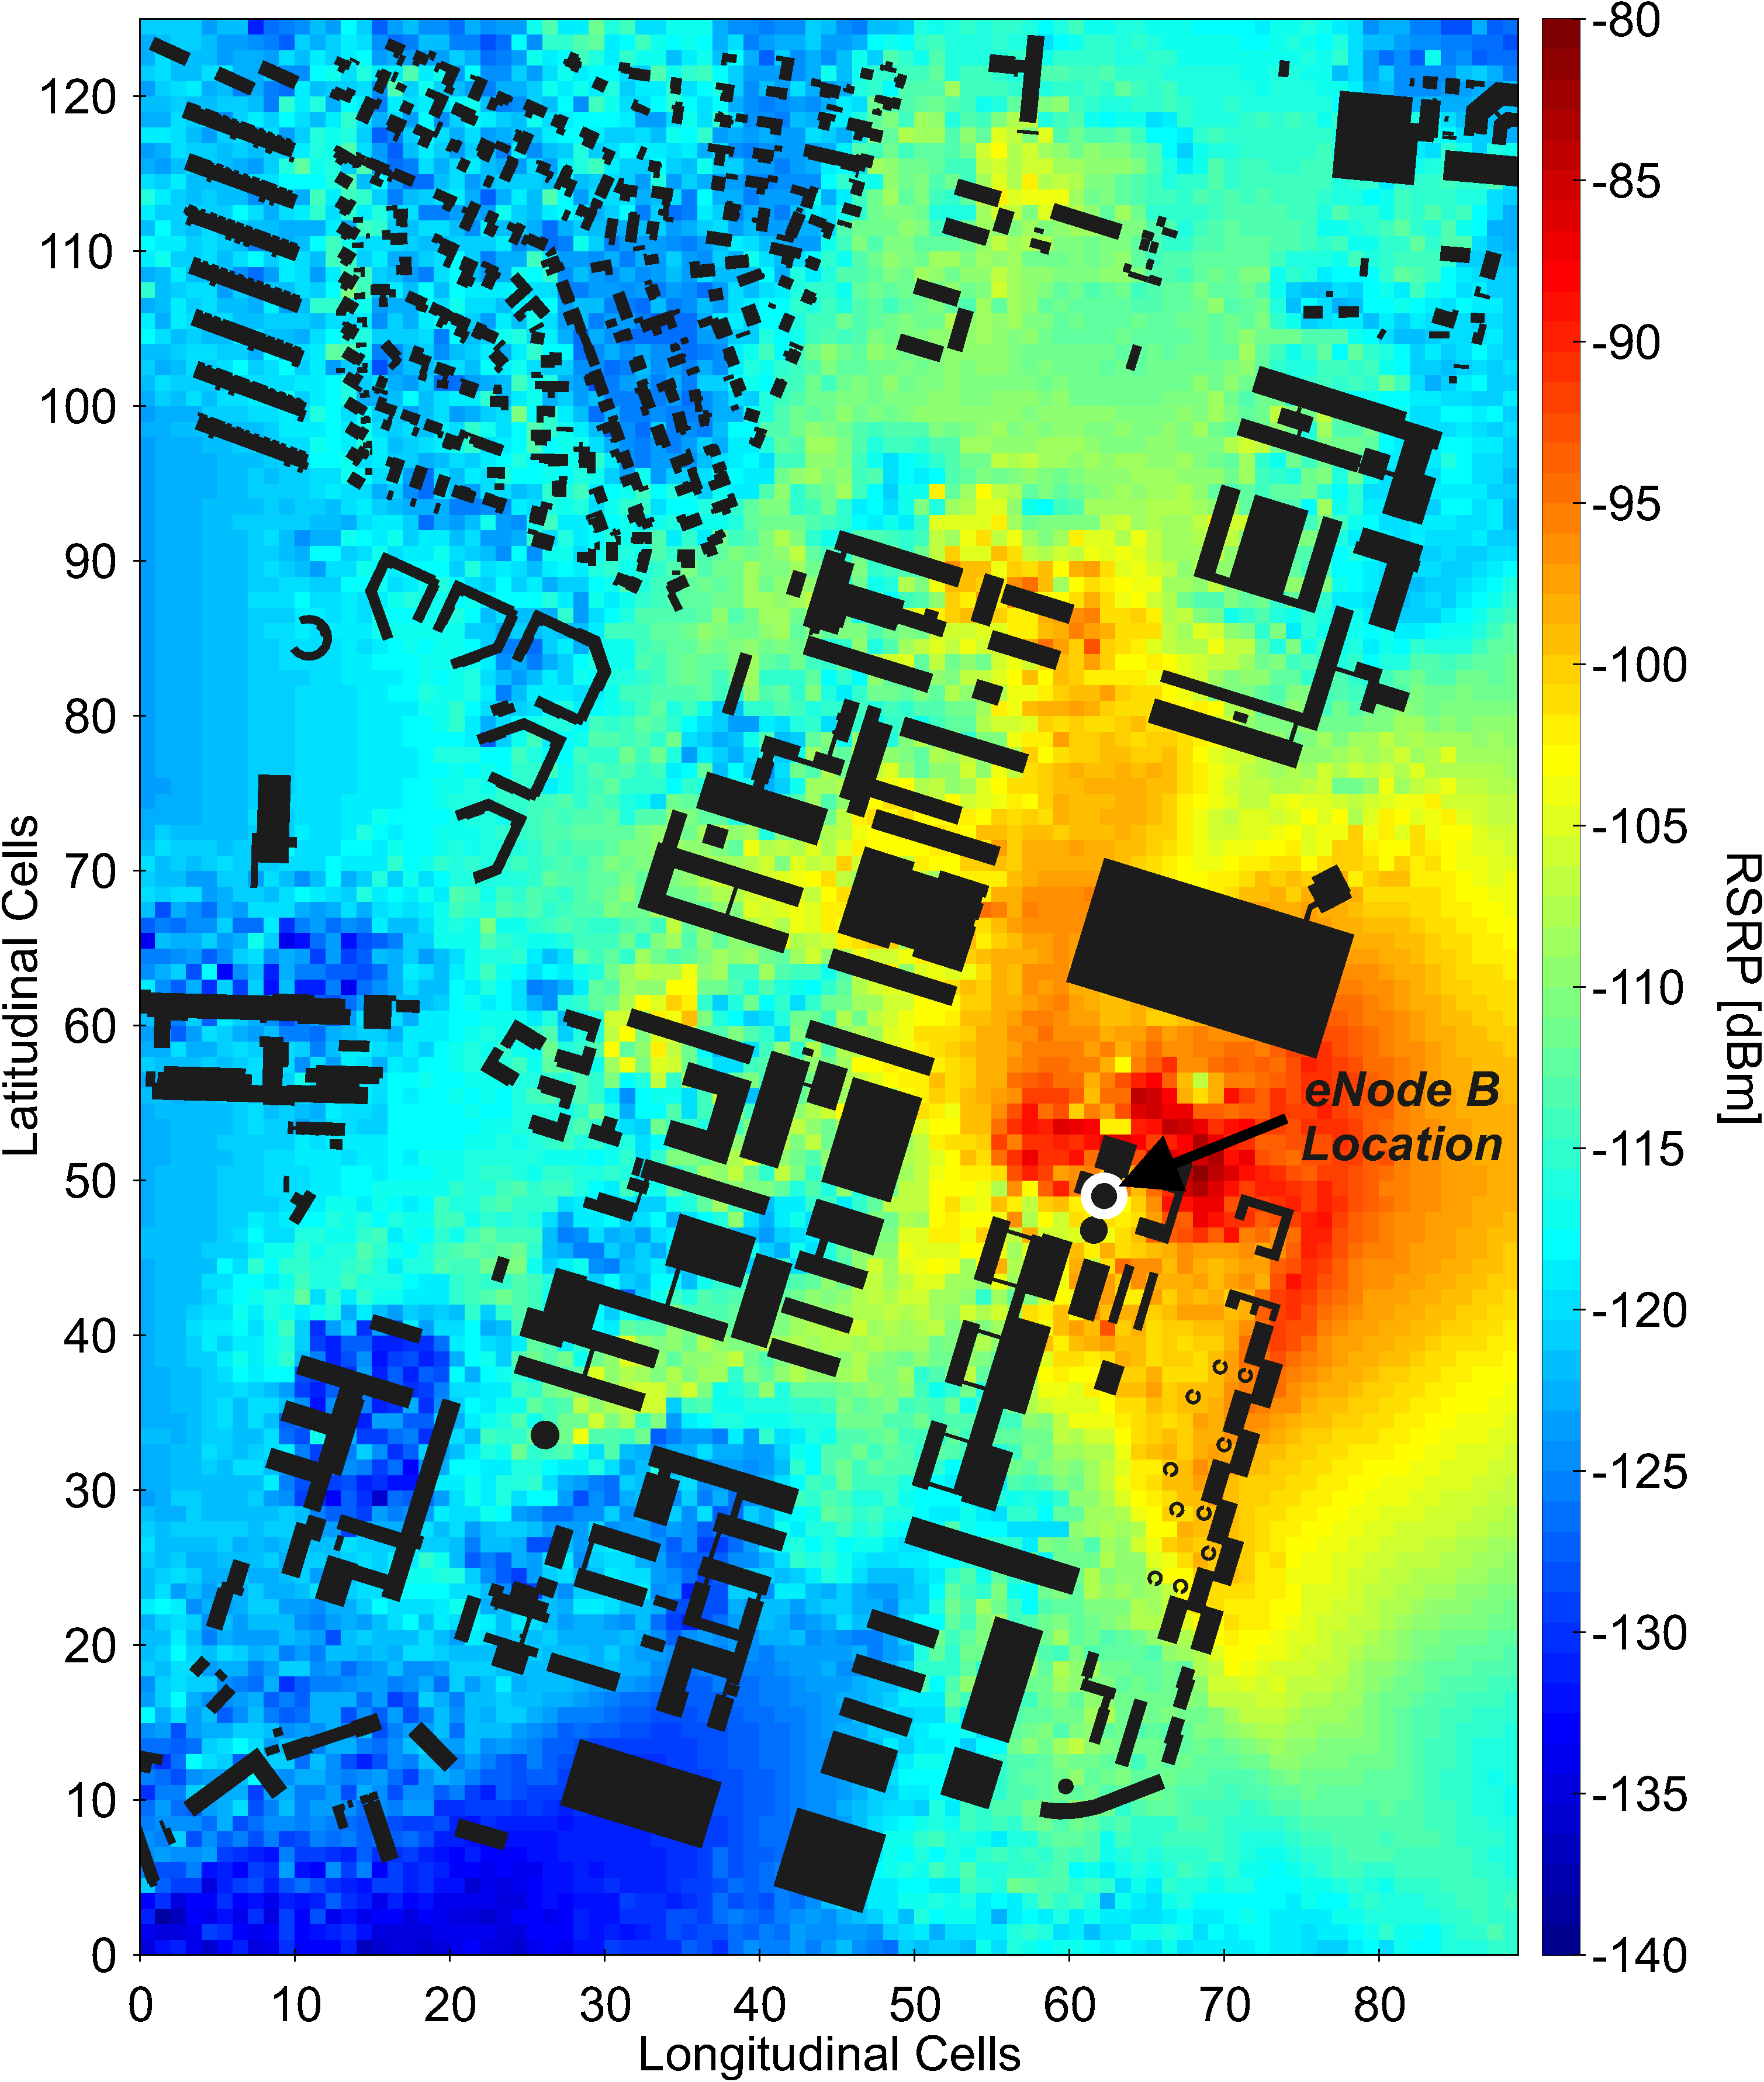
\includegraphics{chapters/part_pathloss/osm_images_paper/figures/heatmap.pdf}
    \caption{Extrapolated heatmap at 2630 MHz using generated features for all latitude and longitude coordinate pairs.}
    \label{fig:osm_heatmap}
\end{figure}

\subsection{Discussion}

A necessary procedure of the proposed method is experimental validation from inherently different data sources. The above-documented results contribute towards such a validation. The use of the German-based datasets is an essential first step in showing the properties and gains of the proposed method. The German-based datasets consist of several frequencies not present in the original \texttt{DK} dataset. More so, it effectively doubles the number of available samples for learning. The procedure for generating the geographical images is simplified as it only requires \gls{osm} data. 

The generalization performance has been analyzed using a cross-validation approach. A necessity of this approach is multiple trained models which is contingent on feasible training times. Evaluating the \texttt{DK Campus} subset is effectively extrapolation across data with an inherently different origin. The results indicate that the generalization across datasets with different data origin is possible and offer accurate performance $\text{\gls{rmse}} = 7.8$ dB. However, by including data from different origins the accuracy is effectively improve as is indicated by the performance $\text{\gls{rmse}} = 6.3$ dB of the \texttt{GER Campus} scenario. The  \texttt{GER Campus} is the campus of TU Dortmund, which does share many architectural similarities with the \texttt{DK Campus} scenario. The results indicate that this is inferred from data with a different origin. 

The geographical images supplied by a \gls{osm} pipeline have effectively resulted in a simplified training procedure and a significant reduction in hyper-parameters. Even with the reduction of hyper-parameters, the original reported gains (as seen in \emph{v2} and \cite{Thrane020ModelAidedDeepLearning}) on the \texttt{DK Campus} dataset are maintained. A direct result of this reduction is the main driver for the cross-validation procedure to be completed in a feasible time. The training time, with over double the amount of samples and a lower batch-size, is maintained at approximately $120$ minutes. The inference time is halved to sub-millisecond predictions.

The produced heatmap offers insight into the predictive capabilities of the method. Even though the heatmap is produced on the scenario at which it was trained, it still had to infer \gls{rsrp} for non-measured locations. The fact that the range of \gls{rsrp} values is within expected values is a favourable property of the trained \gls{nn}. Furthermore, the heatmap shows an increased intensity around the location of the \gls{enb}, which is probably. Finally, some sectorization of the \gls{enb} can, with some imagination, be observed. Future work of the methodology is not only to further test the generalization properties but also the performance to existing methods of producing radiomaps, for instance, compare the proposed approach to that of \emph{Kriging}.

% Altitude information embedding
Additionally, the images contain only information on the building footprints. It would be of great interest to study the embedding of altitude and height information into such images. 


\subsection{Conclusion}\label{subsec:conclusion_v3}
Simple geographical images, along with expert knowledge supply strong prior information for predicting \gls{rsrp} for unseen locations. It is shown that latent features for describing local radio characteristics can be found using simple geographical images. The proposed approach is vigorously validated on additional experimental data. The images were produced using a simplified pipeline utilizing \gls{osm} data and contain only information on buildings and the location. Images spanning a distance of $250-300$ meters was found to produce improved performance. The results show that the proposed method is able to generalize across inherently different data origins. The best predictive performance on an unseen propagation scenario is reported to be $\text{\gls{rmse}} = 6.3$ ($\sigma = 3.6$ dB) on a multitude of operating frequencies.

